%\section{Anforderungen}
%\textit{In diesem Abschnitt soll die Demoanwendung vorgestellt werden, anhand dessen das Proof-of-Concept erstellt wird. Damit das Proof-of-Concept erstellt werden kann, muss die Demoanwendung die zuvor beschriebenen Probleme aufweisen, hierbei sollen die Probleme möglichst realitätsnah sein und nicht frei erfunden.}

Wie in \autoref{anf:1020} beschrieben, ist eine Demoanwendung zu erstellen, auf Basis dessen das Konzept anzuwenden ist und somit praktisch umgesetzt werden kann. Dieser Abschnitt beschäftigt sich mit der Vorstellung der Demoanwendung und der repräsentativen Aufgabe, die diese übernimmt.

In der Motivation wurde ein konkretes Problem eines Kunden der Open Knowledge genannt. Damit die Demoanwendung realistisch eine moderne Webanwendung darstellt, wird sie in Grundzügen die Webanwendung des Direktversicherers nachahmen. Bei der Webanwendung handelt es sich um einen Wizard, also einer Sequenz von aufeinanderfolgenden Dialogseiten bei dem der Nutzer Daten eingeben soll. Die ist zum Großteil clientseitig abgebildet und eine mit Angular erstellte SPA. Die Webanwendung validiert einzelne Felder gegen Partnersysteme (bspw. beim Adressfeld). Am Ende des Wizard werden die gesamten Daten an ein weiteres Partnersystem übermittelt, welches darauf basierend eine Berechnung durchführt und das Ergebnis dann an die Webanwendung sendet.

Es wurde sich dafür entschieden, dass die Webanwendung eine Bestellfunktionalität eines Obst-Webshops darstellen soll. Der Warenkorb hierfür wird anfangs dynamisch generiert und dies soll so simulieren, dass eine andere Komponente diesen erstellt hat. Der Nutzer soll seine Rechnungs- und Lieferdaten eingeben und am Ende die Bestellung ausführen können. Um das gewünschte Verhalten der Demoanwendung zu definieren, wird es im folgenden Abschnitt festgelegt.

\subsection{Verhaltensdefinition}

Mit den beiden Stakeholdern, also Christian Wansart und Stephan Müller, die beide am Projekt für den Kunden involviert sind, wurde diese Verhaltensdefinition erstellt. Diesen Ansatz der Definition der Software anhand des Verhaltens nennt man Behavior-Driven Development (BDD). BDD wurde 2006 erstmals von Dan North benannt und definiert \cite{IntroducingBDD}. Bei BDD werden User-Stories aus der Sicht eines äußerlichen Betrachters entworfen und geschrieben. Dabei umfassen die User-Stories Beispiele, wie die Anwendung in diesen Szenarien sich verhalten soll.

Um die BDD-Definition festzuhalten wurde sie in der gängigen Gherkin-Syntax \cite{Gherkin} geschrieben. Die Syntax ist natürlich zu lesen, folgend werden alle gewünschten Features der Demoanwendung in der Gherkin-Syntax aufgelistet.

\lstinputlisting[
  language = gherkin,
   caption = Demoanwendung: Gherkin Definition zum Feature \enquote{Warenkorb},
captionpos = b,
     label = lst:demoanwendung-gherkin-warenkorb
]{content/04_erstellung-poc/warenkorb-gherkin/1-warenkorb.feature}

\lstinputlisting[
  language = gherkin,
   caption = Demoanwendung: Gherkin Definition zum Feature \enquote{Rechnungsadresse},
captionpos = b,
     label = lst:demoanwendung-gherkin-rechnungsadresse
]{content/04_erstellung-poc/warenkorb-gherkin/2-rechnungsadresse.feature}

\lstinputlisting[
  language = gherkin,
   caption = Demoanwendung: Gherkin Definition zum Feature \enquote{Lieferadresse},
captionpos = b,
     label = lst:demoanwendung-gherkin-lieferadresse
]{content/04_erstellung-poc/warenkorb-gherkin/3-lieferadresse.feature}

\lstinputlisting[
  language = gherkin,
   caption = Demoanwendung: Gherkin Definition zum Feature \enquote{Zahlungsdaten},
captionpos = b,
     label = lst:demoanwendung-gherkin-zahlungsdaten
]{content/04_erstellung-poc/warenkorb-gherkin/4-zahlungsdaten.feature}

\lstinputlisting[
  language = gherkin,
   caption = Demoanwendung: Gherkin Definition zum Feature \enquote{Bestellung abschließen},
captionpos = b,
     label = lst:demoanwendung-gherkin-bestellung_abschließen
]{content/04_erstellung-poc/warenkorb-gherkin/5-bestellung_abschließen.feature}

Neben des eigentlichen User-Interfaces soll auch ein Backend teil der Demoanwendung sein. Hierfür wurde auf Basis der Verhaltensdefinition eine Architektur entworfen, die im folgenden Abschnitt näher beschrieben wird.

\subsection{Backend}

Das Backend wurde als Microservice-Architektur konzipiert und wurde ebenso wie die Webanwendung auch an das Projekt des Open Knowledge Kunden angelehnt. In \autoref{fig:demoanwendung_deployment} lässt sich die konzipierte und umgesetzte Architektur betrachten, hierbei stellen Pods einzelne Containersysteme dar. Diese Architektur wurde mit den Stakeholdern zusammen konzipiert und ähnelt dem des Direktversicherers.

Für das Frontend ist die einzig anzusprechende Schnittstelle das \enquote{backend4frontend}, welches die Kommunikation zu Partnersysteme ermöglicht und welches Sicherheits- und Validitätsaspekte überprüft. Die weiteren Dienste \enquote{Bestellungen}, \enquote{Übersetzungen}, \enquote{Addressvalidierung} und \enquote{Warenkorb} übernehmen die jeweilige Funktion, die ihr Name beschreibt. Der Dienst \enquote{Bestellungen} ist das Partnersystem, welches beim Fertigstellen des Wizards aufgerufen wird und dabei führt es weitere Datenabfragen und Validitätsüberprüfungen durch.

Durch diese recht komplexe Architektur kann eine realitätsnahe Repräsentation erfolgen. Speziell wird bei einer solchen Architektur Tracing hilfreicher, um die Zusammenhänge zwischen den Diensten nachvollziehen zu können. Dies wird beim Einsatz und der Vorstellung der Lösung näher betrachtet.

% Die einzelnen Dienste sind als Java EE Microservices umgesetzt worden und dabei minimal gehalten worden. 

\begin{figure}[H]
	\centering
	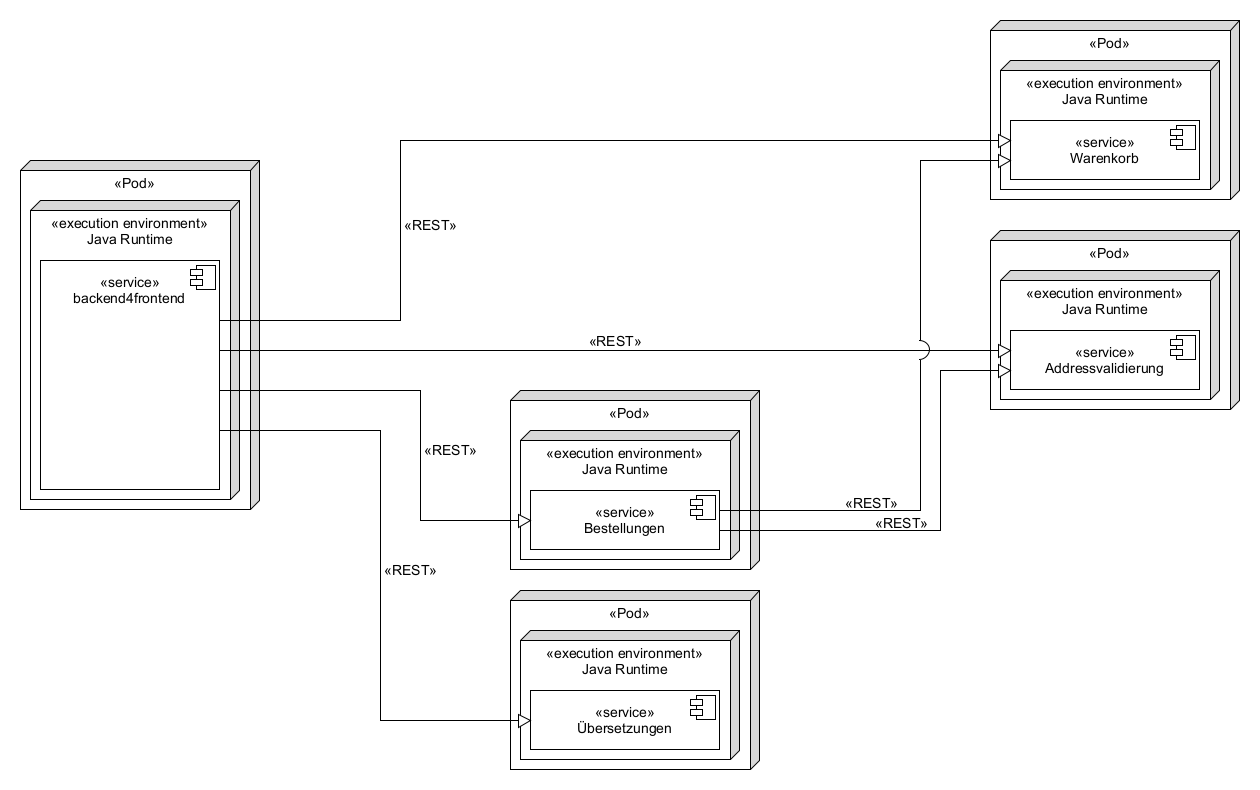
\includegraphics[width=1.0\linewidth]{img/04_erstellung-poc/demoanwendung_deployment.png}
	\caption{Demoanwendung: Deployment-Diagramm, Quelle: Eigene Darstellung}
	\label{fig:demoanwendung_deployment}
\end{figure}

\subsection{Frontend}

Wie beim Direktversicherer wurde ein Wizard auf Basis von Angular erstellt, welcher als zustandsreiche SPA umgesetzt ist. In den folgenden Abbildungen \ref{fig:demoanwendung_vorstellung_01-warenkorb} -- \ref{fig:demoanwendung_vorstellung_06-bestellbestaetigung} wird das Frontend anhand einer Beispieldurchlaufs vorgestellt.

Wie in \autoref{anf:1020} definiert wurden in das Frontend einige Fehler eingebaut, damit diese, mit der zu erstellenden Lösung, aufgedeckt werden können. Diese Fehler werden näher im nachfolgenden \autoref{subsec:fehlerszenarien} betrachtet.

\begin{figure}[H]
	\centering
	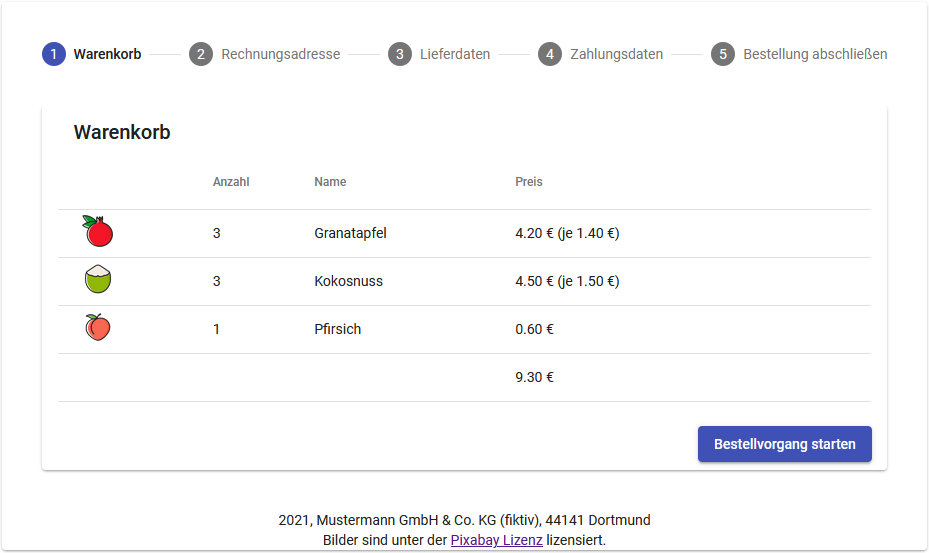
\includegraphics[width=0.75\linewidth]{img/04_erstellung-poc/demoanwendung_vorstellung_01-warenkorb.png}
	\caption{Demoanwendung: Startseite \enquote{Warenkorb}}
	\label{fig:demoanwendung_vorstellung_01-warenkorb}
\end{figure}

\begin{figure}[H]
	\centering
	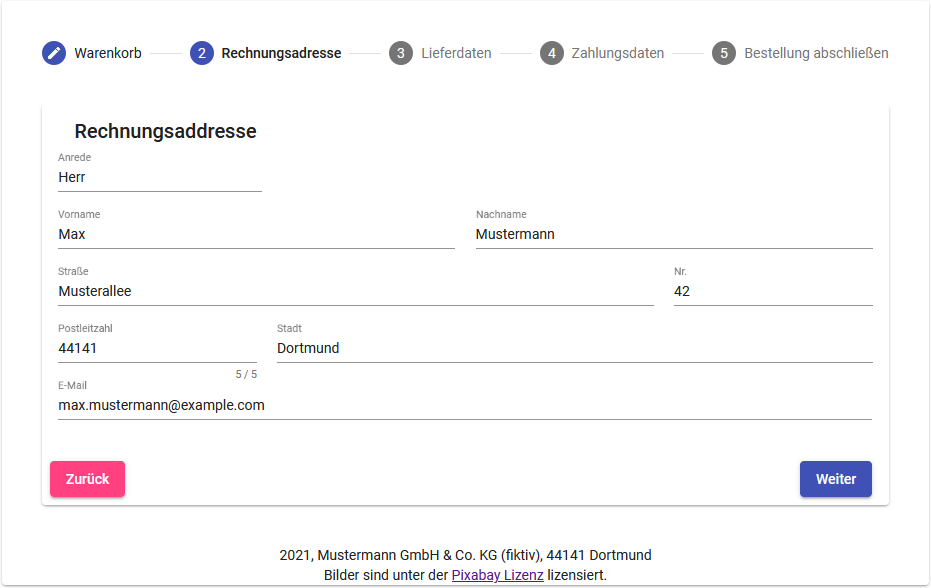
\includegraphics[width=0.75\linewidth]{img/04_erstellung-poc/demoanwendung_vorstellung_02-rechnungsadresse.png}
	\caption{Demoanwendung: Seite \enquote{Rechnungsadresse}}
	\label{fig:demoanwendung_vorstellung_02-rechnungsadresse}
\end{figure}

\begin{figure}[H]
	\centering
	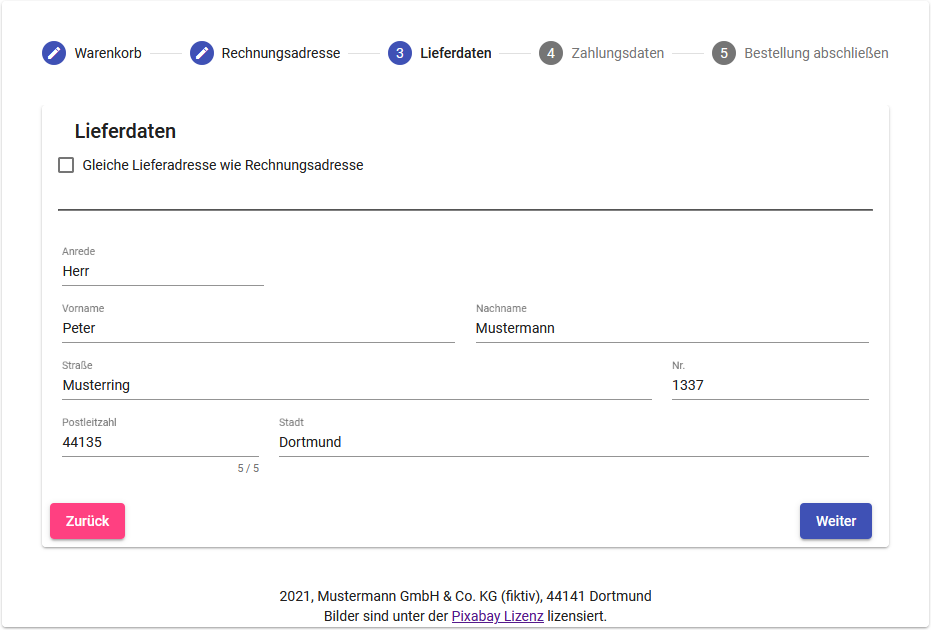
\includegraphics[width=0.75\linewidth]{img/04_erstellung-poc/demoanwendung_vorstellung_03-lieferdaten.png}
	\caption{Demoanwendung: Seite \enquote{Lieferdaten}}
	\label{fig:demoanwendung_vorstellung_03-lieferdaten}
\end{figure}

\begin{figure}[H]
	\centering
	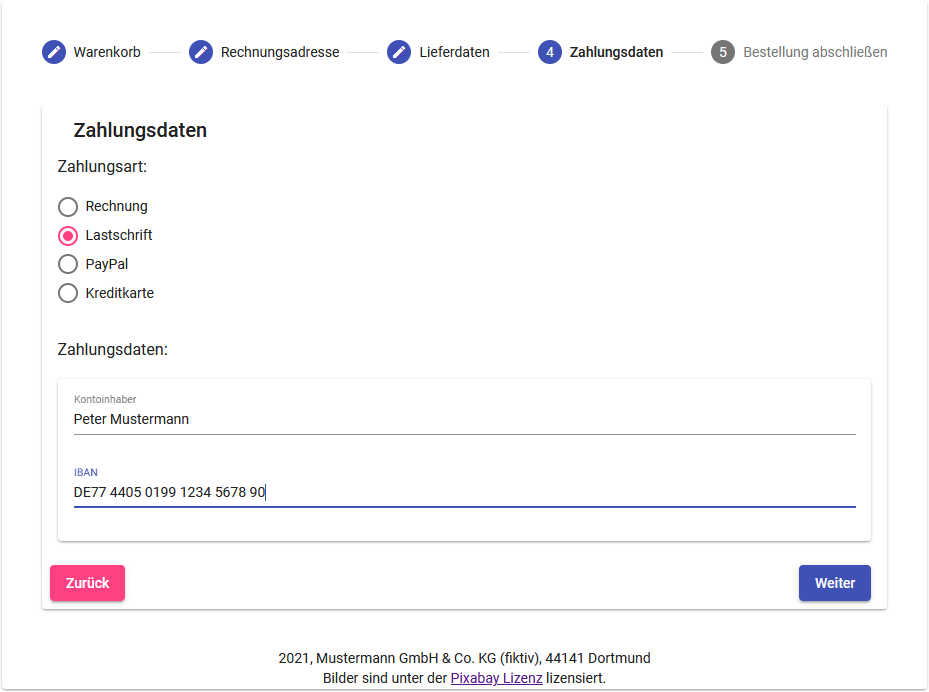
\includegraphics[width=0.75\linewidth]{img/04_erstellung-poc/demoanwendung_vorstellung_04-zahlungsdaten.png}
	\caption{Demoanwendung: Seite \enquote{Zahlungsdaten}}
	\label{fig:demoanwendung_vorstellung_04-zahlungsdaten}
\end{figure}

\begin{figure}[H]
	\centering
	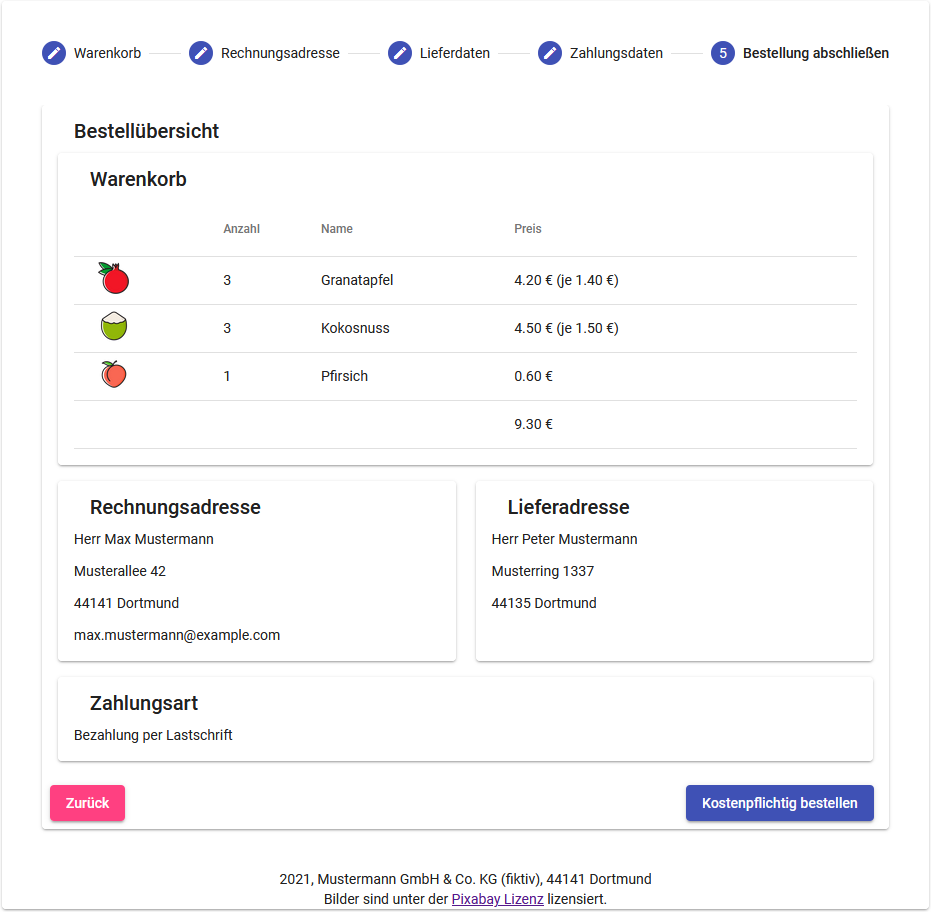
\includegraphics[width=0.75\linewidth]{img/04_erstellung-poc/demoanwendung_vorstellung_05-bestelluebersicht.png}
	\caption{Demoanwendung: Seite \enquote{Bestellübersicht}}
	\label{fig:demoanwendung_vorstellung_05-bestelluebersicht}
\end{figure}

\begin{figure}[H]
	\centering
	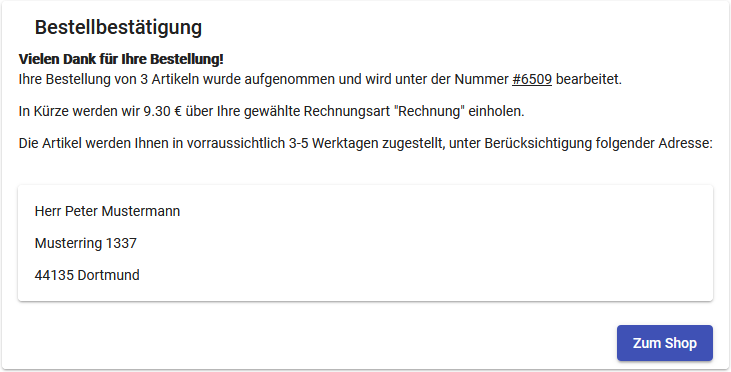
\includegraphics[width=0.75\linewidth]{img/04_erstellung-poc/demoanwendung_vorstellung_06-bestellbestaetigung.png}
	\caption{Demoanwendung: Finale Seite \enquote{Bestellbestätigung}}
	\label{fig:demoanwendung_vorstellung_06-bestellbestaetigung}
\end{figure}

\subsection{Fehlerszenarien}
\label{subsec:fehlerszenarien}

Wie zuvor erwähnt und in \autoref{anf:1020} gewünscht, besitzt die Demoanwendung einige simulierte Fehler. Diese Fehler wurden in Zusammenarbeit mit den Stakeholdern konzipiert. Bei der Konzeption wurde versucht möglichst realitätsnahe oder sogar tatsächlich beim Kunden aufgetretene Probleme einzubauen.

Diese Fehler gehören unterschiedlichen Problemgruppen an, sie reichen von unerwünscht strenger Validierung, über Konfigurationsfehlern bis hin zu ineffizienter Datenverarbeitung. Sie werden folgen in Fehlerszenarien beschrieben, aus der Sicht eines Projektteams, welches diese Szenarien berichtet bekommen oder selbst notiert hat.

\subsubsection{\enquote{Keine Übersetzungen}}

\begin{wrapfigure}[6]{r}{0.33\textwidth}
\centering
\vspace{-\baselineskip}
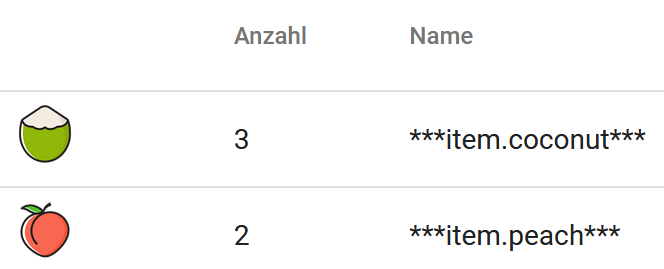
\includegraphics[width=\linewidth]{img/04_erstellung-poc/demoanwendung_fehlerszenario-uebersetzungen}
\caption{Fehlende Texte}
\label{fig:demoanwendung_fehlerszenario-uebersetzungen}
\end{wrapfigure}

- Problem: Nutzer berichten, dass manchmal die Webanwendung beim Start keine Artikeltexte anzeigt (vgl \autoref{fig:demoanwendung_fehlerszenario-uebersetzungen}).

- Ursache: Die Pods, die den Übersetzungsdienst enthalten werden repliziert bereitgestellt. Einer der Pods hat eine defekte Konfiguration, weswegen er keine Übersetzungen der Artikel enthält. Wird zu diesem Pod verbunden, tritt das Fehlverhalten auf. Dies ist eine Nachstellung eines tatsächlichen Problems beim Kunden.

\subsubsection{\enquote{Gültige Straßen sind ungültig}}

- Problem: Nutzer berichten, dass Ihr Straßenname nicht eingeben werden kann. Beispielsweise die Eingabe \enquote{Ährenweg} führt zu einem Fehler.

- Ursache: Der Adressvalidierungsdienst validiert Straßen mit dem RegEx \texttt{[a-zA-Z\textbackslash,\textbackslash-\textbackslash ]+}, welches keine gängigen Sonderzeichen (ä ,ö ,ü, ß) erlaubt.

\subsubsection{\enquote{Gültige Hausnummern sind ungültig}}

- Problem: Nutzer berichten, dass Hausnummern, die nicht nur aus Zahlen bestehen, zum Fehler führen.

- Ursache: Der Adressvalidierungsdienst validiert Hausnummern als Zahl und schlägt im o. g. Fall in der Konvertierung fehl.

\subsubsection{\enquote{Gültige Städte sind ungültig}}

- Problem: Nutzer aus Gießen berichten, dass Sie das Formular zur Rechnungsadresse nicht ausfüllen können

- Ursache: Der Adressvalidierungsdienst meldet die Stadt \enquote{Gießen} als ungültig, weil sie nicht in der lokalen Tabelle vorhanden ist.

\subsubsection{\enquote{Ungültige Adressen sind gültig}}

- Problem: Nutzer können in den Lieferdaten ungültige Eingaben tätigen und absenden, bei der Bestellaufgabe kommt es zu einem Fehler.

- Ursache: Das Frontend überprüft lediglich die Rechnungsadresse, aber nicht die Lieferadresse

\subsubsection{\enquote{Vor- und Nachnamen werden abgeschnitten}}

- Problem: Nutzer berichten, dass in der Bestellbestätigung Ihre Vor- und Nachnamen abgeschnitten dargestellt werden.

- Ursache: Der Bestelldienst begrenzt den Vor- sowie den Nachnamen auf 20 Zeichen.

\subsubsection{\enquote{Falsche Zahlungsart}}

- Problem: Nutzer berichten, dass in der Bestellbestätigung die falsche Zahlungsart angezeigt wird. In der Bestellübersicht wurde jedoch die korrekte Zahlungsart angezeigt.

- Ursache: Das Frontend sendet alle Formulardaten an Bestelldienst, dieser nimmt aber an, dass alle nicht ausgewählten Formulare \texttt{null} sind.

\subsubsection{\enquote{Lange Verarbeitung}}

- Problem: Beim Absenden des Formulars auf der Seite \enquote{Warenkorb} kommt es zu einer unerwünschten Wartezeit (von min. 6-10s).

- Ursache: Dies ist eine simulierte Wartezeit im Frontend je nach Anzahl der Positionen (2s pro Position), um eine ineffiziente Verarbeitung nachzuahmen.

\subsection{Repräsentation}

Eine wichtige Eigenschaft der Demoanwendung sollte sein, dass sie repräsentativ für die Webanwendung des Kunden ist und im Allgemeineren auch für moderne Webanwendungen ist. Durch den groben Aufbau der Demoanwendung, also einer zustandsreichen und zu großen Teilen clientbasierten SPA, stellt die Demoanwendung eine moderne Webanwendung dar. Auch die Verwendung von Angular ist repräsentativ, denn Angular ist eines der meist verwendeten Frontend-Frameworks \cite{TheStateOfJavaScript2020}.

Das Backend ist in dem Sinne repräsentativ, dass es auf keiner stark vereinfachten Infrastruktur basiert, sondern gewollt an die Sitatuation des Open Knowledge Kunden abbildet. Des Weiteren stellt die gewählte Architektur einen modernen Ansatz dar, denn die Architektur ist Microservice-orientiert\cite{MicroserviceArchitecture}.

Dennoch ist anzumerken, dass die Demoanwendung nur ein Modell einer tatsächlichen Webanwendung darstellt. Wie jedes Modell können nicht alle Gegebenheiten des zu modellierenden Sachverhalts nachgestellt werden. Jedoch ist durch den allgemein gehaltenen Anwendungsfall und die moderne Umsetzung eine Übertragbarkeit zu ähnlichen Projekten durchaus vorhanden.

Nun da die Demoanwendung beschrieben ist, wird das Konzept erstellt, welches letztendlich auf die Demoanwendung anzuwenden ist. Das Konzept selber ist jedoch losgelöst von der Demoanwendung zu verstehen.